%!TEX root = ../dissertation.tex
\chapter{Introduction}
\label{introduction}

\indent The Standard Model of Elementary Particles (SM) provides a concrete description of the interactions and dynamics of all known elementary particles with the exception of gravity.  In the SM, matter is composed of three generation of fermions with spin 1/2 while interactions are governed by gauge symmetries and mediated by spin 1 gauge bosons.  \\

\indent The last piece of the SM, the Higgs boson, was discovered in 2012 at the Large Hadron Collider.  The complex scalar Higgs field spontaneously breaks the electroweak (EW) symmetry by acquiring a vacuum expectation value (VEV). This process of electroweak symmetry breaking (EWSB) gives mass to the $W$ and $Z$ gauge bosons. The fermions also acquire their mass through Yukawa interactions between the Higgs and fermion fields. \\

\indent Although the Brout-Englert-Higgs mechanism ensure that the SM theory will remain viable as a perturbative physical theory up to the Planck scale, current experimental evidence suggests that the SM is not a complete theory of nature.  SM leaves several important fundamental questions unanswered.  These open questions include but is not limited to the nature of Dark Matter (DM), the apparent matter/anti-matter asymmetry in the universe,  the reason behind the SM mass spectrum, the potential unification of EW and strong interactions at high energy scales, the nature of neutrino mass and the hierarchy problem regarding the naturalness of the Higgs mass.  The answers to these questions are at the frontier of physics research and form the major physics goals of many different physics experiments across multiple disciplines. \\

\indent One proposed solution to many of these questions is the introduction of a new spacetime symmetry called supersymmetry.  Supersymmetry imposes a new symmetry between fermions and bosons allowing one to transform into the other.  In this way, the supersymmetric extension to the SM (SUSY) predicts the existence of a yet undiscovered superpartner to every known SM particle.  The SM particles and their respective superpartners are shown in figure \ref{fig:SUSYpart} \\

\begin{figure}[h!]
%\begin{center}
\centering
    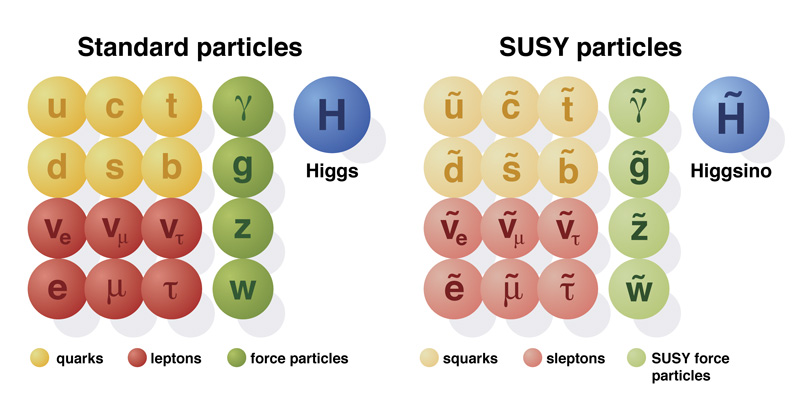
\includegraphics[width=0.85\textwidth]{figures/strategy/SUSYparticles.jpg}\hspace{0.05\textwidth}
\caption[Diagram of SM particles and their respective superpartners]{ Diagram of SM particles and their respective superpartners. }
\label{fig:SUSYpart}
%\end{center}
\end{figure}

\indent SUSY gives one possible solution to the hierarchy problem of the Higgs as large contributions to the Higgs potential are canceled out between SM particles and their superpartners.  Some supersymmetric models also unify the strong and electroweak force at high energies, provide more cp violation to generate matter/antimatter asymmetry and produce plausible dark matter candidates.  At the same time, general relativity is automatically included if SUSY is imposed as a local symmetry. This offers a potential path to uniting general relativity with quantum mechanics.  \\

\indent All previous high energy experiments including the Tevatron and LEP have not detected the existence of superpartners.  Therefore, if SUSY exists in nature then it must be a spontaneously broken symmetry.  Many different SUSY symmetry-breaking mechanisms have been proposed but they all make the superpartners more massive then their SM counterparts. \\

\indent A major goal of the Large Hadron Collider (LHC) experiment is to search for the predicted superpartners at an unprecedented energy scale.  If SUSY is the solution to the hierarchy problem and restores naturalness to the Higgs mechanism then the superpartner to the top quark (stop) is expected to be no heavier then a few $\tev$.  The stop's mass is strongly constrained due to the large coupling between the SM top quark and the Higgs with $\lambda_t \sim 0.94$.  As such, searches for the stop at the LHC is especially interesting because the stop's mass may be low enough to be directly produced at the energy scale of the LHC. \\

\indent This thesis concerns the search for stops in an traditionally experimentally difficult region.  One expected stop decay channel produces a top quark along with the superpartner to a neutral electroweak boson, the neutralino (\ninoone).  The Feynman diagram for stop production and decay is shown in figure \ref{fig:stopprod}. \\

\begin{figure}[h!]
%\begin{center}
\centering
    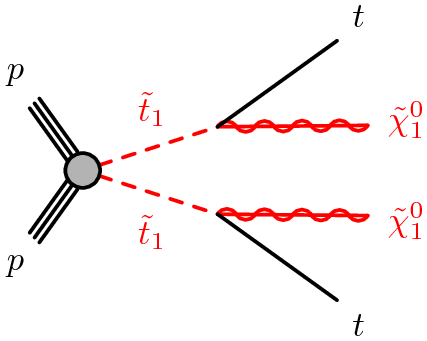
\includegraphics[width=0.45\textwidth]{figures/feynDiag/stst-tN1tN1.png}\hspace{0.05\textwidth}
\caption[Feynman diagram for the production and decay of stops at the LHC]{ Feynman diagram for the $pp \rightarrow \stop\stop \rightarrow t\ninoone t\ninoone$ process.  This process is one of the expected stop production and decay channels at the LHC.  The $\stop \rightarrow t\ninoone$ decay channel can have large branching fractions if the lightest stop is mainly right-handed or the lightest supersymmetric particle is a bino. The exact branching fraction depends on the sparticle masses in the SUSY model and whether the lightest stop is mainly right or left-handed. }
\label{fig:stopprod}
%\end{center}
\end{figure}

\indent One popular search strategy for stops targets the experimental signatures of neutralinos as they are unique to SUSY.  Experimentally this involves searching for events with large missing transverse energy ($\met$), the experimental signature of high momentum neutralinos.  This search strategy can effectively detect stops if there is a large mass splitting between $m_{\stop}$ and $m_{\ninoone}$. The heavy stop can impart large amounts of momentum onto its decay products in this region of phase space.  Monte Carlo simulation of the $\met$ distribution for the $m_{\stop} = 1000 \gev$ and $m_{\ninoone} = 1 \gev$ signal is shown as the dashed yellow histogram in figure \ref{fig:presel:MET}.  The $\met$ distribution for SM backgrounds can also be seen in the solid stacked histogram.  \\

\begin{figure}[h!]
%\begin{center}
\centering
    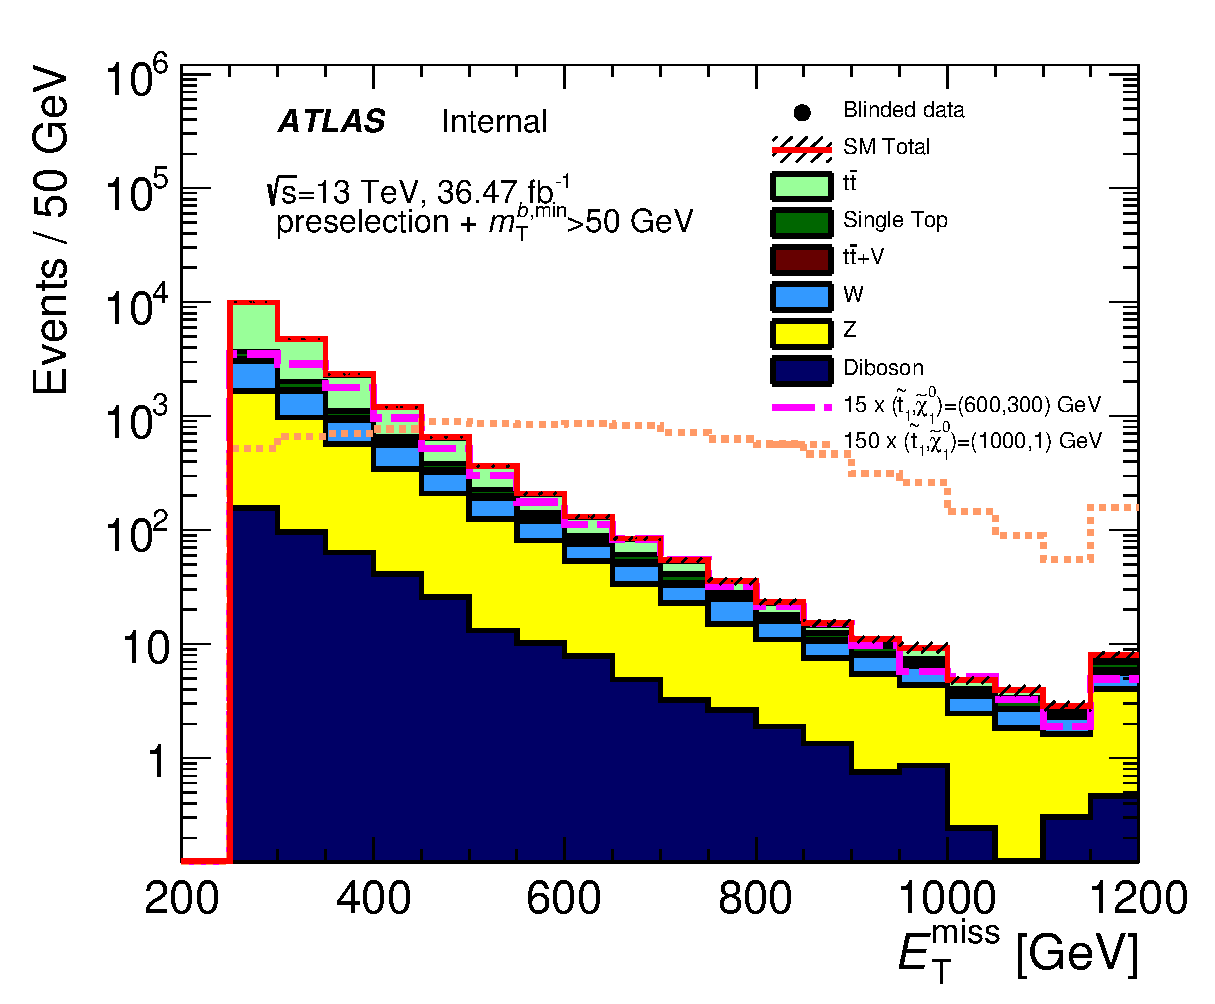
\includegraphics[width=0.85\textwidth]{figures/preselection/Met_preCutSRPlot_withRatio_log.eps}\hspace{0.05\textwidth}
\caption[Stop signal with $m_{\stop}-m_{\ninoone} >> m_t$ and SM background $\met$ distribution after loose preliminary selections for $\met>250 \gev$, zero leptons and at least four jets]{ $\met$ distribution for $(m_{\stop}, m_{\ninoone}) = (1000 \gev,1 \gev)$ and $(600 \gev, 300 \gev)$ stop signal and expected SM background.  The signal cross section has been scaled up by 150 and 15 respectively for better visibility.  Basic selections ensuring well reconstructed $\met$, no leptons, and at least four jets are applied.  Details on selections can be found in \cite{stop0LCONF} }
\label{fig:presel:MET}
%\end{center}
\end{figure}

\indent The $\met$ distribution for the $m_{\stop} = 600 \gev$ and $m_{\ninoone} = 300 \gev$ signal can also be seen in figure \ref{fig:presel:MET} as the dashed purple histogram.  The smaller mass splitting between stop and neutralino in the (600 \gev,300 \gev) sample means the stop has less energy to boost the heavy neutralino.  This leads to a softer $\met$ distribution and less separation power between signal and background.  \\

\indent   When the stop mass is nearly degenerate to $m_t + m_{\ninoone}$ the stop has just enough energy to produce the top and neutralino.  The resulting stop decay products gain little momenta from the stop decay. The low $\pt$ neutralinos in turn generate very little $\met$.  The $\met$ distribution for $(m_{\stop}, m_{\ninoone}) = (250 \gev,77 \gev)$, $(300 \gev, 127 \gev)$ and $(400 \gev, 227 \gev)$ signal samples is given in figure \ref{fig:presel:MET_diag}.  As we can see, the $\met$ variable provides little separation power between signal and background in this region of phase space. \\

\begin{figure}[h!]
%\begin{center}
\centering
    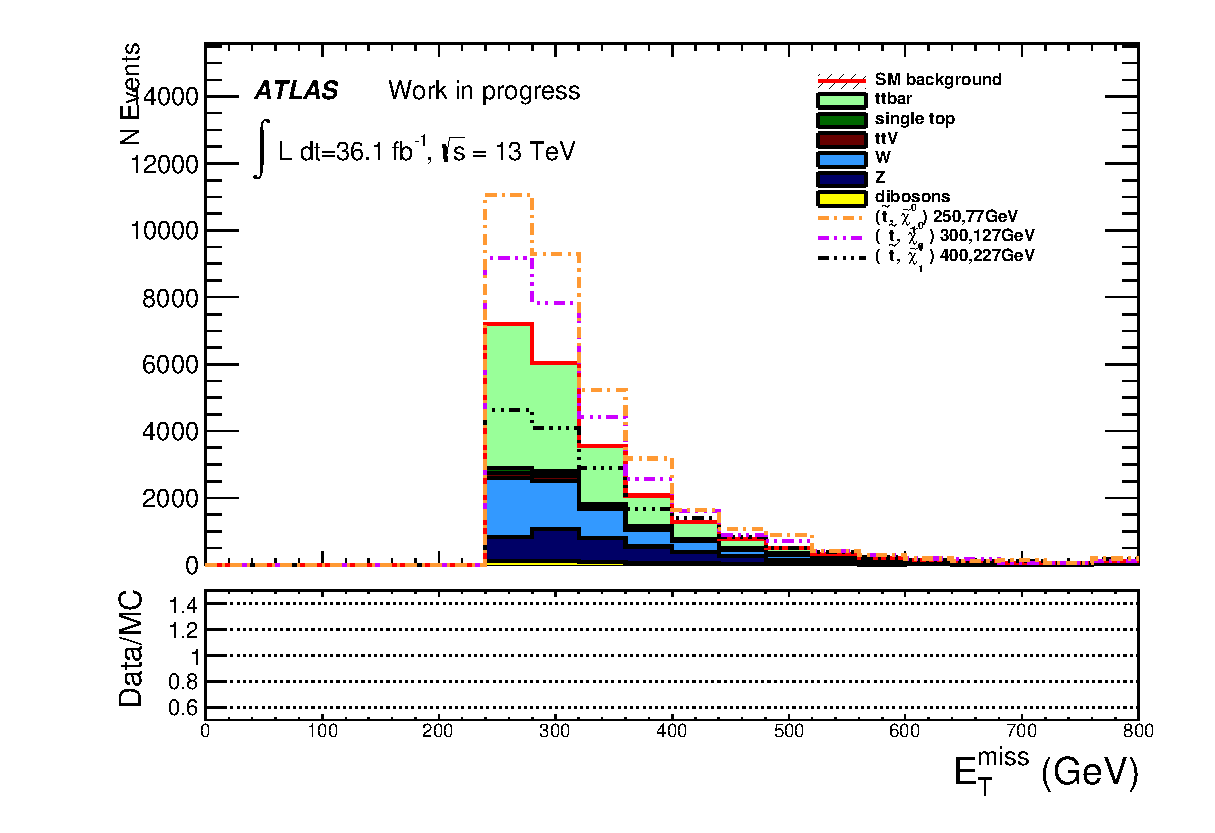
\includegraphics[width=0.85\textwidth]{figures/plotSR/SR_eT_miss_0SR.eps}\hspace{0.05\textwidth}
\caption[Stop signal with $m_{\stop}-m_{\ninoone} \sim m_t$ and SM background $\met$ distribution after loose preliminary selections for $\met>250 \gev$, zero leptons and at least four jets]{ $\met$ distribution for $(m_{\stop}, m_{\ninoone}) = (250 \gev,77 \gev)$, $(300 \gev, 127 \gev)$ and $(400 \gev, 227 \gev)$ stop signal and expected SM background.  All three signal samples have $m_{\stop}-m_{\ninoone} \sim m_t$.  The signal cross section has also been scaled up by a factor of 20 for better visibility.  Basic selections ensuring well reconstructed $\met$, no leptons, and minimal jet multiplicity requirements are applied.  Preselections are defined in chapter \ref{chap:Selection_EventPreselection} }
\label{fig:presel:MET_diag}
%\end{center}
\end{figure}

\indent The only other observables in the event are the visible tops which are also produced in SM top/anti-top pair (ttbar) production.  This inability to distinguish SM ttbar from stop signal greatly hamper the search sensitivity in this region because SM ttbar production cross section is 50$\times$ to 300$\times$ that of the stop . \\

\indent The low decay product $\pt$ problem is ubiquitous to all regions of phase space with small mass splittings.  Many ATLAS searches in SUSY including charginos, Higgsinos, sbottom, sleptons, etc all have some region of phase space with a compressed mass spectra.  In general, such regions of phase space are called compressed regions. \\

\indent The ATLAS Run 1 stop search results are summarized in figure \ref{fig:ATLAS:8TeVResult}.  Shaded regions have been excluded by ATLAS Run 1 searches to 95\% confidence.  The different colored regions correspond to different searches.  \\

\begin{figure}[h!]
%\begin{center}
\centering
    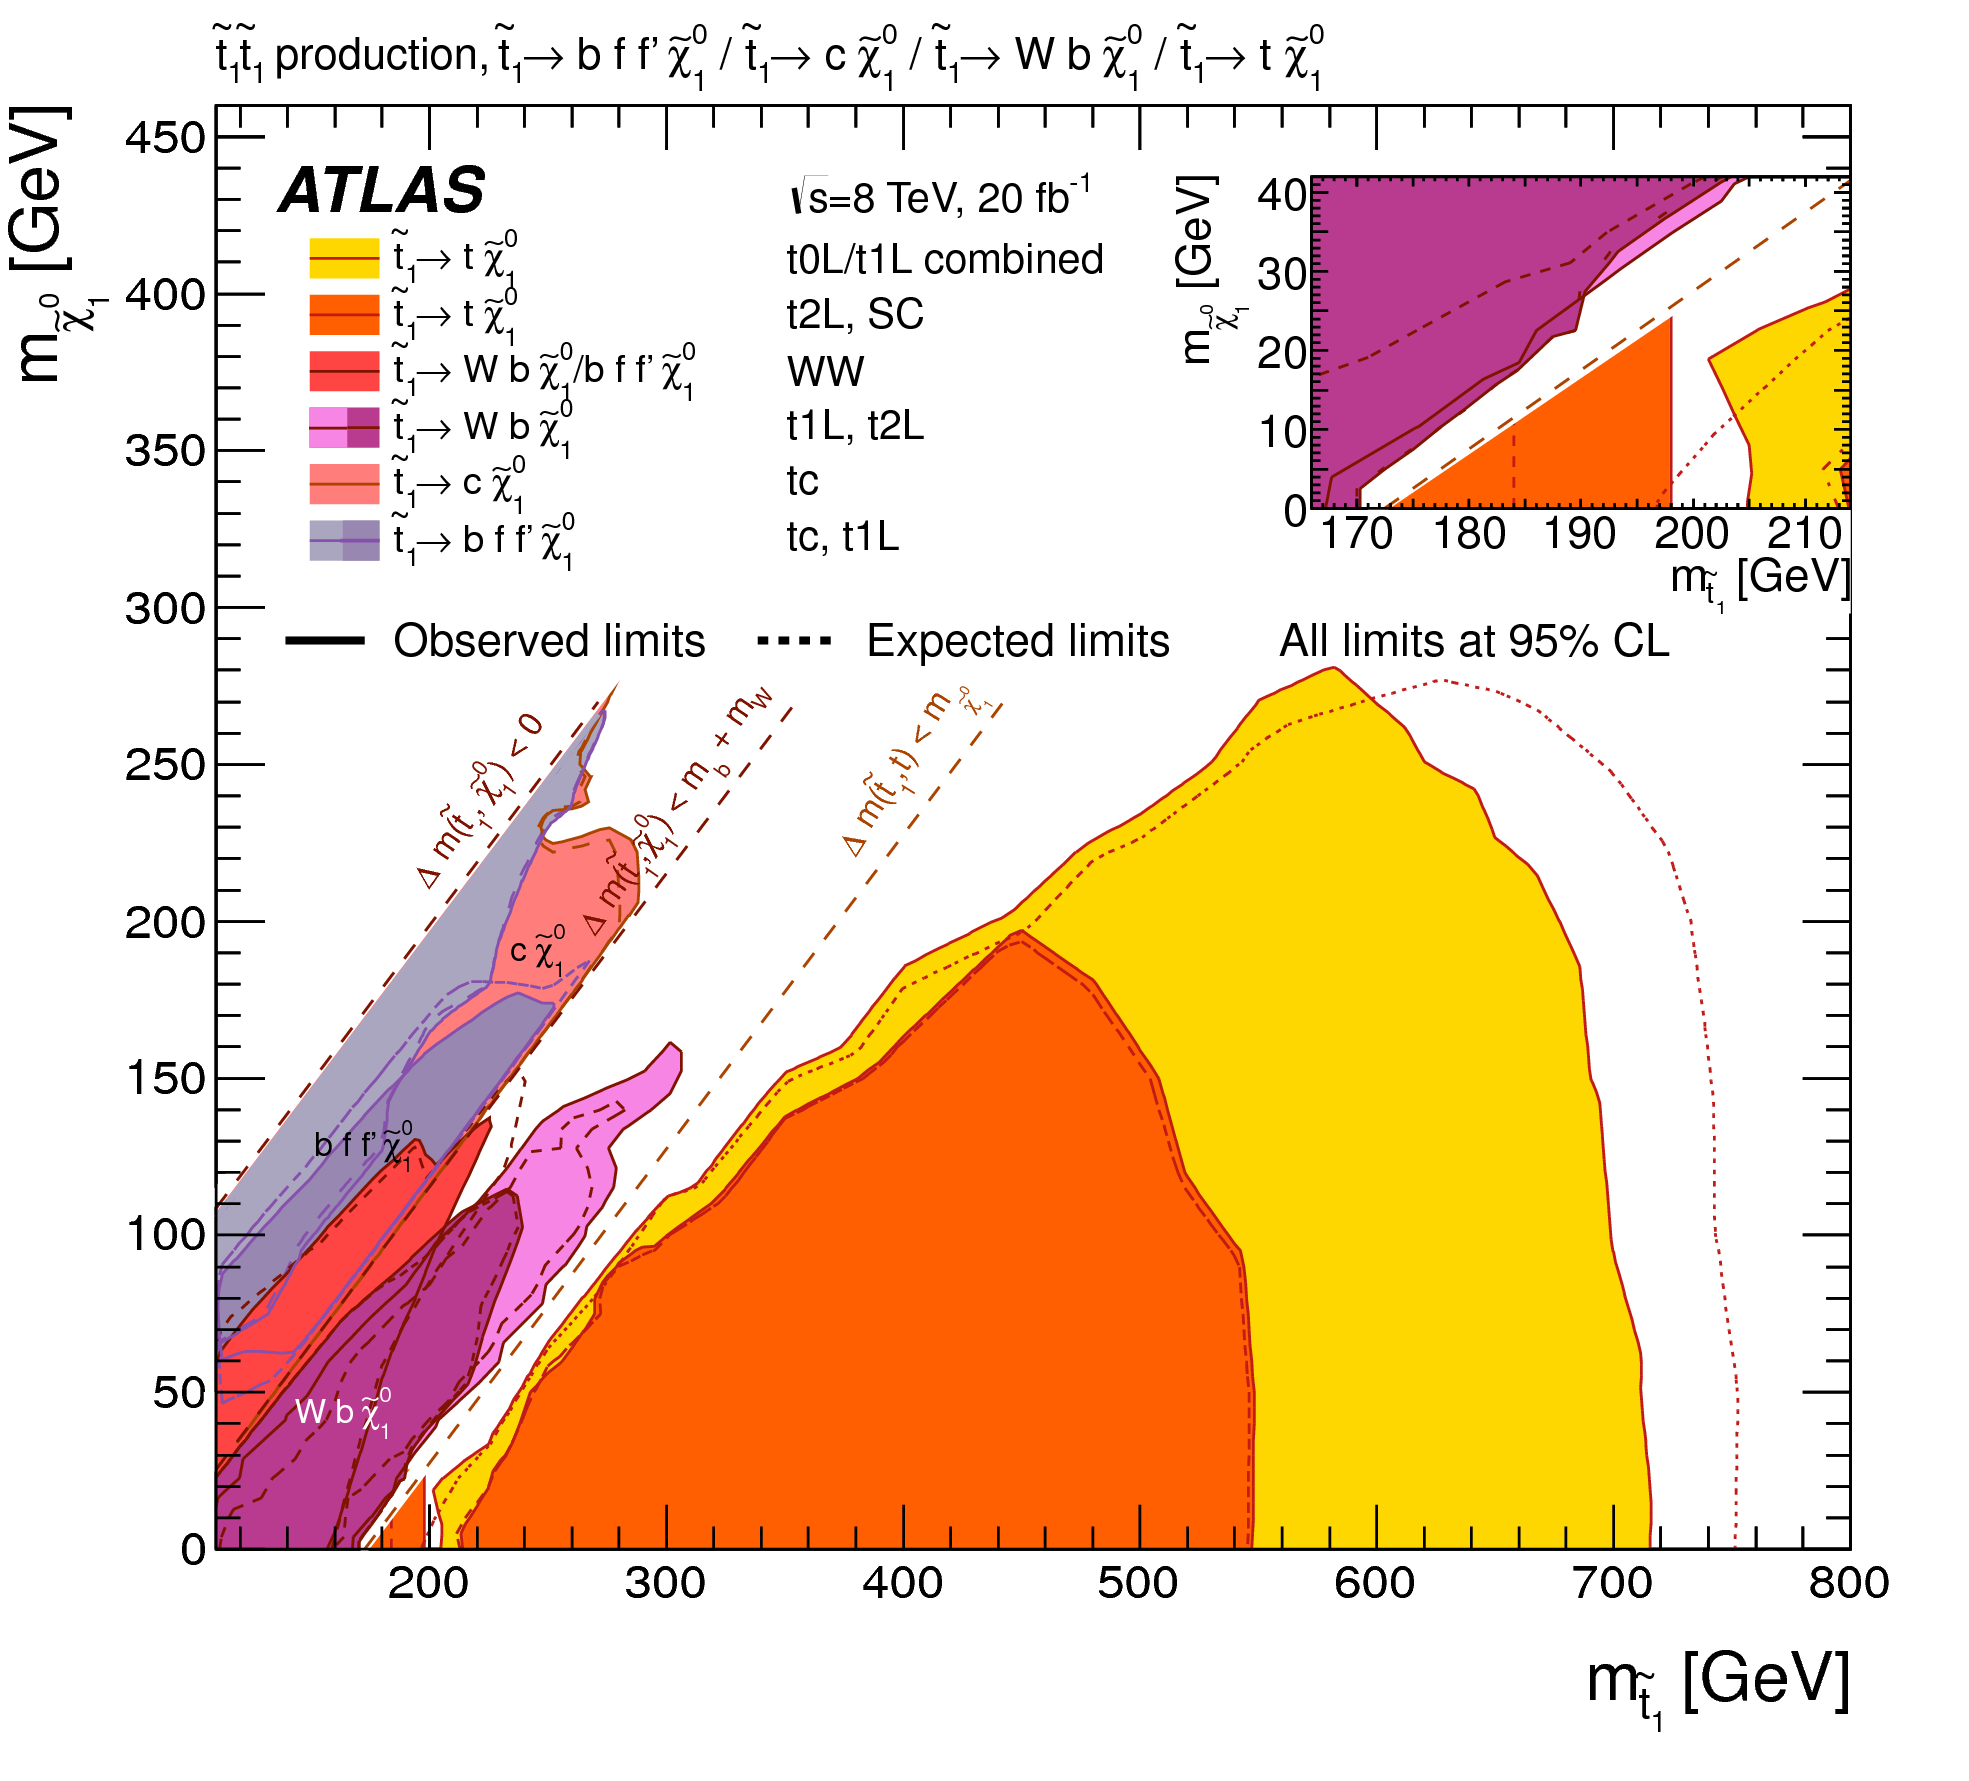
\includegraphics[width=0.85\textwidth]{figures/8TeV/ATLAS_SUSY_Stop_tLSP_201507.png}\hspace{0.05\textwidth}
\caption[95\% confidence limits on stop parameter space from various analysis on ATLAS $\sqrt{s} = 7+8 \tev$ data]{ 95\% confidence limits on stop parameter space from various analysis on ATLAS $\sqrt{s} = 7+8 \tev$ data.  Shaded regions have been excluded by ATLAS Run 1 searches.  Different colored regions correspond to different search strategies including different experimental signatures. The $m_{\stop}-m_{\ninoone} = m_t$ remains unconstrained for all stop masses. }
\label{fig:ATLAS:8TeVResult}
%\end{center}
\end{figure}

\indent Searches targeting high $\met$ is sensitive to stop signals with large mass splittings at the bottom right corner. Searches targeting off shell top decays are sensitive to regions with mass splittings smaller than the top mass ($m_{\stop}-m_{\ninoone} < m_t$).  These searches are able to rule out the purple, red and gray regions above the $m_{\stop}-m_{\ninoone} = m_t$ diagonal line.  However, the corridor near $m_{\stop}-m_{\ninoone} = m_t$ remain unconstrained even at low stop masses.  The same features can be seen in Run 1 CMS results shown in figure \ref{fig:CMS:8TeVResult}. \\

\begin{figure}[h!]
%\begin{center}
\centering
    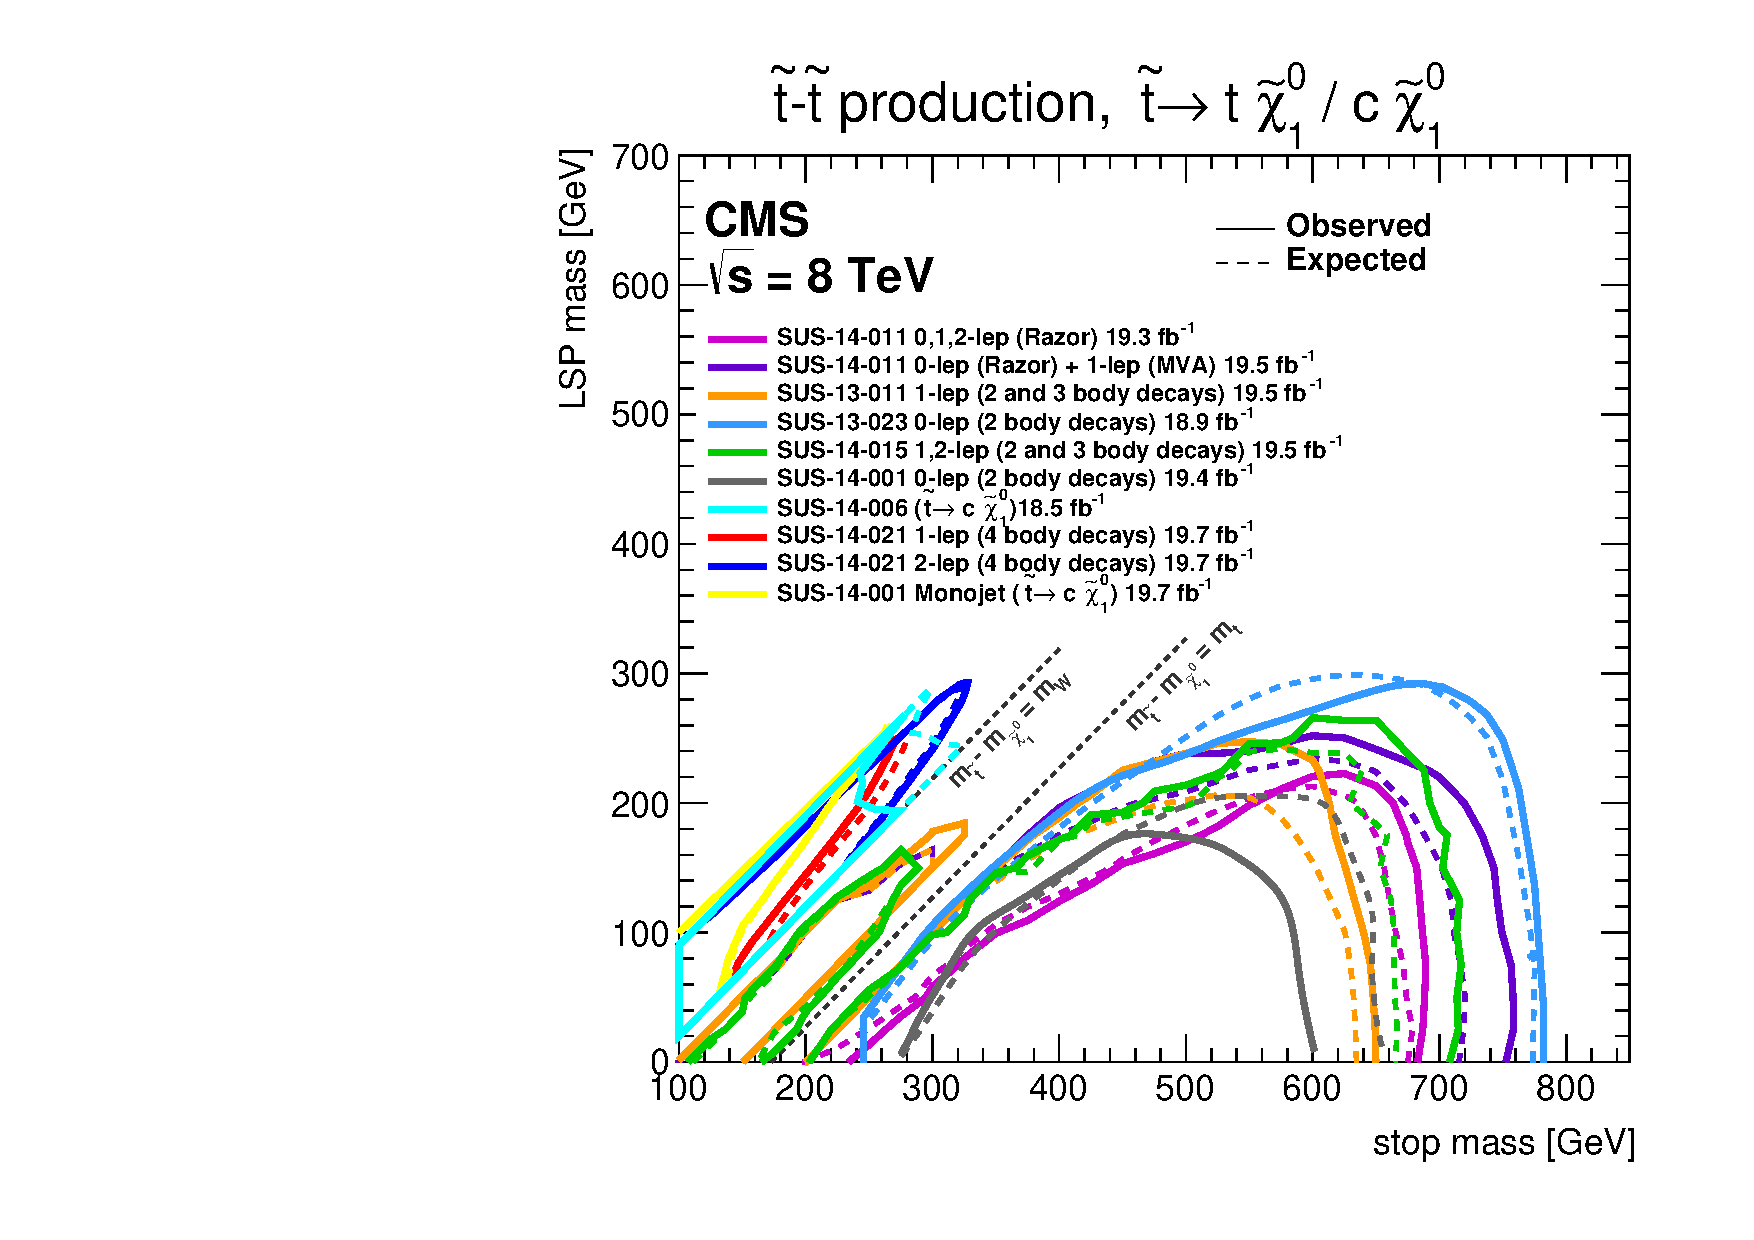
\includegraphics[width=0.85\textwidth, angle=270]{figures/8TeV/T2tt_2015.pdf}\hspace{0.05\textwidth}
\caption[95\% confidence limits on stop parameter space from various analysis on CMS $\sqrt{s} = 7+8 \tev$ data]{ 95\% confidence limits on stop parameter space from various analysis on CMS $\sqrt{s} = 7+8 \tev$ data.  Regions below colored curves have been excluded by CMS Run 1 searches.  Different colored curves correspond to different search strategies including different experimental signatures. The $m_{\stop}-m_{\ninoone} = m_t$ line remains unconstrained for all stop masses.  }
\label{fig:8TeVResult}
%\end{center}
\end{figure}


\indent This thesis demonstrates a new method of searching for stops in the $m_{\stop}-m_{\ninoone} = m_t$ compressed region by isolating events with strong initial state radiation (ISR).  The ISR boosts the stops and gives additional momentum to the stop decay products.  The correlation between ISR pt and stop decay product $\pt$ tend to be extremely strong in this region precisely because the stop decay products gain little momentum from the stop decays.  Specifically there exists a strong correlation between ISR and neutralino systems in both direction and $\pt$.  \\

\indent The neutralinos will inherit a fraction of the original ISR $\pt$ proportional to  $m_{\ninoone}/m_{\stop}$ and the two should be back-to-back.  The $\met/\PTISR$ ratio distribution can be seen in figure \ref{fig:trueRISR}.  The two stop signals both have $m_{\stop}-m_{\ninoone} = m_t$.  Their $\met/\PTISR$ ratios peak sharply at $m_{\ninoone}/m_{\stop}$ according to their respective stop and neutralino masses.  \\

\begin{figure}[h!]
%\begin{center}
\centering
    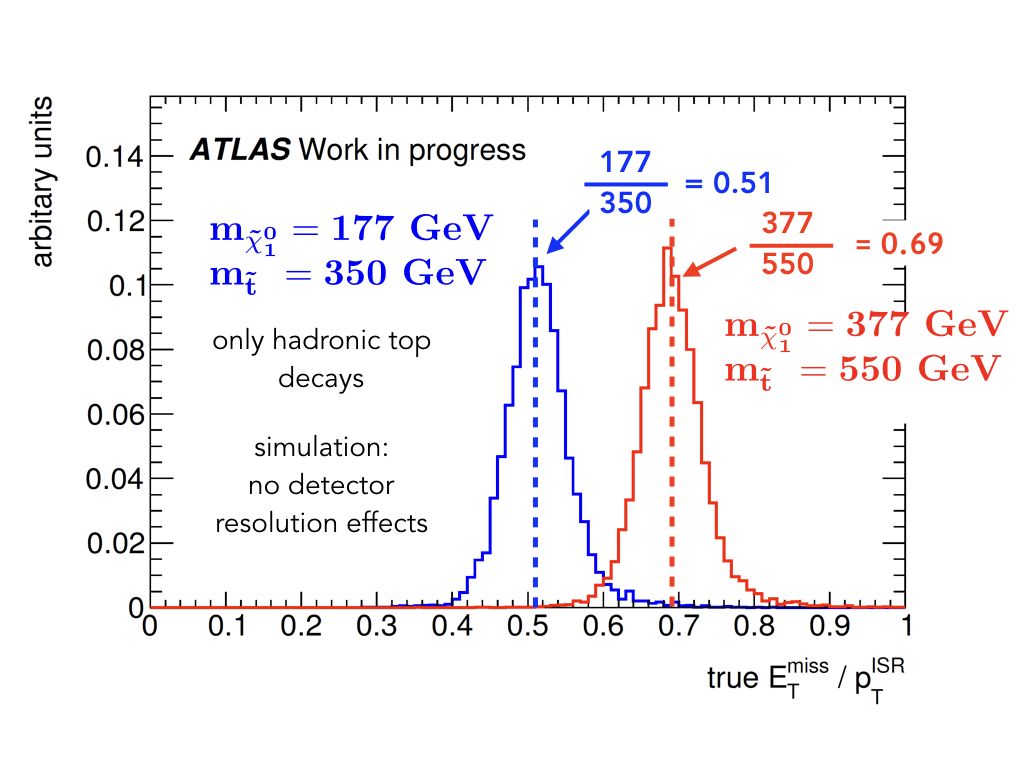
\includegraphics[width=0.85\textwidth]{figures/strategy/RISR_truth.png}\hspace{0.05\textwidth}
\caption[Correlation between the $\met/\PTISR$ ratio in simulation for stop samples with $m_{\stop}-m_{\ninoone} = m_t$]{ Correlation between the $\met/\PTISR$ ratio in simulation for two stop samples with $m_{\stop}-m_{\ninoone} = m_t$.  Both stop samples peak sharply at $m_{\ninoone}/m_{\stop}$ with only a gaussian width of 4 percent.  Deviation from the preferred ratio is limited by the top width, as the top must be pulled off-shell to generate phase space. No detector resolution effects where included and only the all hadronic decay channel was considered. }
\label{fig:trueRISR}
%\end{center}
\end{figure}

\indent These correlations between ISR and $\met$ allow us to separate signal from ttbar background and overcome the difference in production cross section in this experimentally difficult region.  \\

\indent In order to capitalize on these sharply peaking variables, we developed a new accurate ISR identification system.  The algorithm works by first finding the axis of maximum back-to-back $\pt$ call the thrust axis.  The thrust axis should mimic the axis of back-to-back boost between the ISR and sparticle systems in events with strong ISR because the ISR and sparticle boost represents the single largest back-to-back kick in events with strong ISR.  \\

\indent A schematic representation of the thrust axis in stop plus strong ISR events can be seen in figure \ref{fig:ISR:ttbar_sig_example}. \\

\begin{figure}[h!]
  \centering
	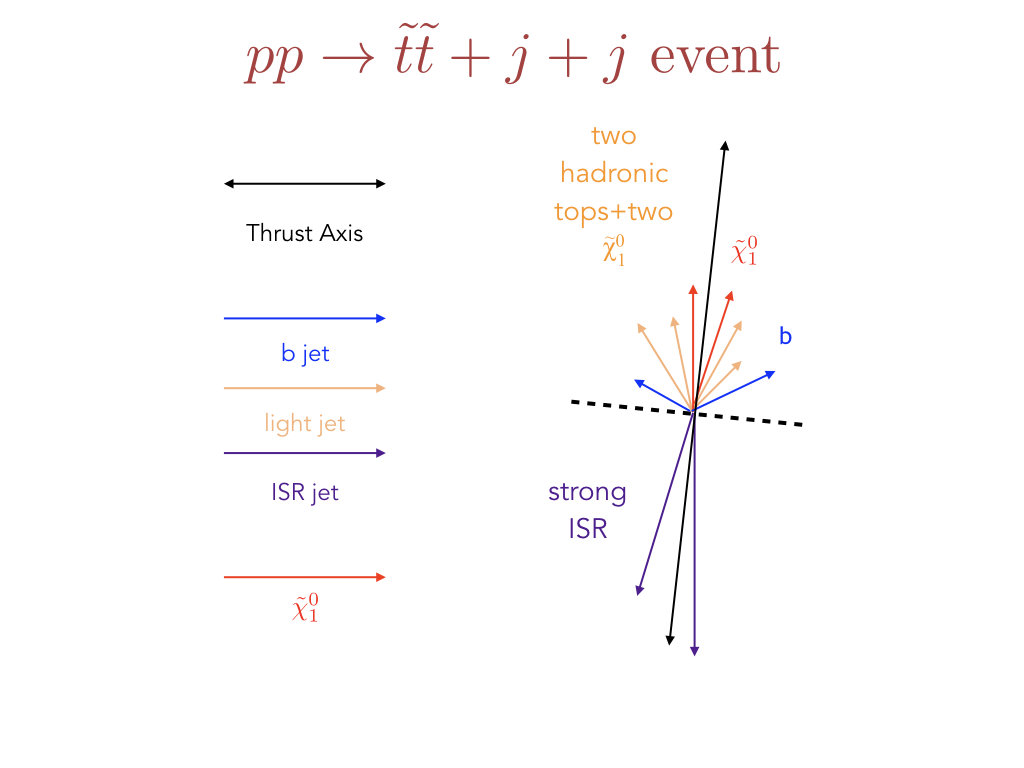
\includegraphics[width=0.85\textwidth]{./figures/strategy/ISR_signal.png}
	\caption[Schematic depictions of stop plus strong initial state radiation event kinematics]{Schematic depictions of stop plus strong ISR event kinematics.  The thrust axis approximates the direction of back-to-back boost between ISR and stop decay products.  The hemisphere containing $\met$ also contains most of the other stop decay products.  The hemisphere opposite the $\met$ contains the energetic ISR jets. }
	\label{fig:ISR:ttbar_sig_example}
\end{figure}

\indent We then divide the event into two hemispheres according to the thrust axis.  All objects in the same hemisphere as the $\met$ are considered to have originated from a stop decay because we expect the neutralinos to travel in the same direction as the original stops.  All objects in the hemisphere opposite the $\met$ are considered to have originated from ISR.  In this way, the thrust-based algorithm is able to identify entire ISR systems composed of multiple jets.  \\ 

\indent The ISR identification algorithm is completely general and can be used to identify ISR for SM processes as well as other BSM searches.  The performance of the ISR identification algorithm in stop and SM ttbar events can be seen in figure \ref{fig:ISRPerformanceIntro}.  In summary, the algorithm can achieve a 9 percent uncertainty on the reconstructed ISR $\pt$ in stop and ttbar events with at least 400 $\gev$ of true ISR $\pt$. This uncertainty includes any detector uncertainties due to the reconstruction of jets, $\met$ and other physics objects.  \\

\begin{figure}[h!]
\centering
    \begin{subfigure}[b]{0.40\textwidth}
    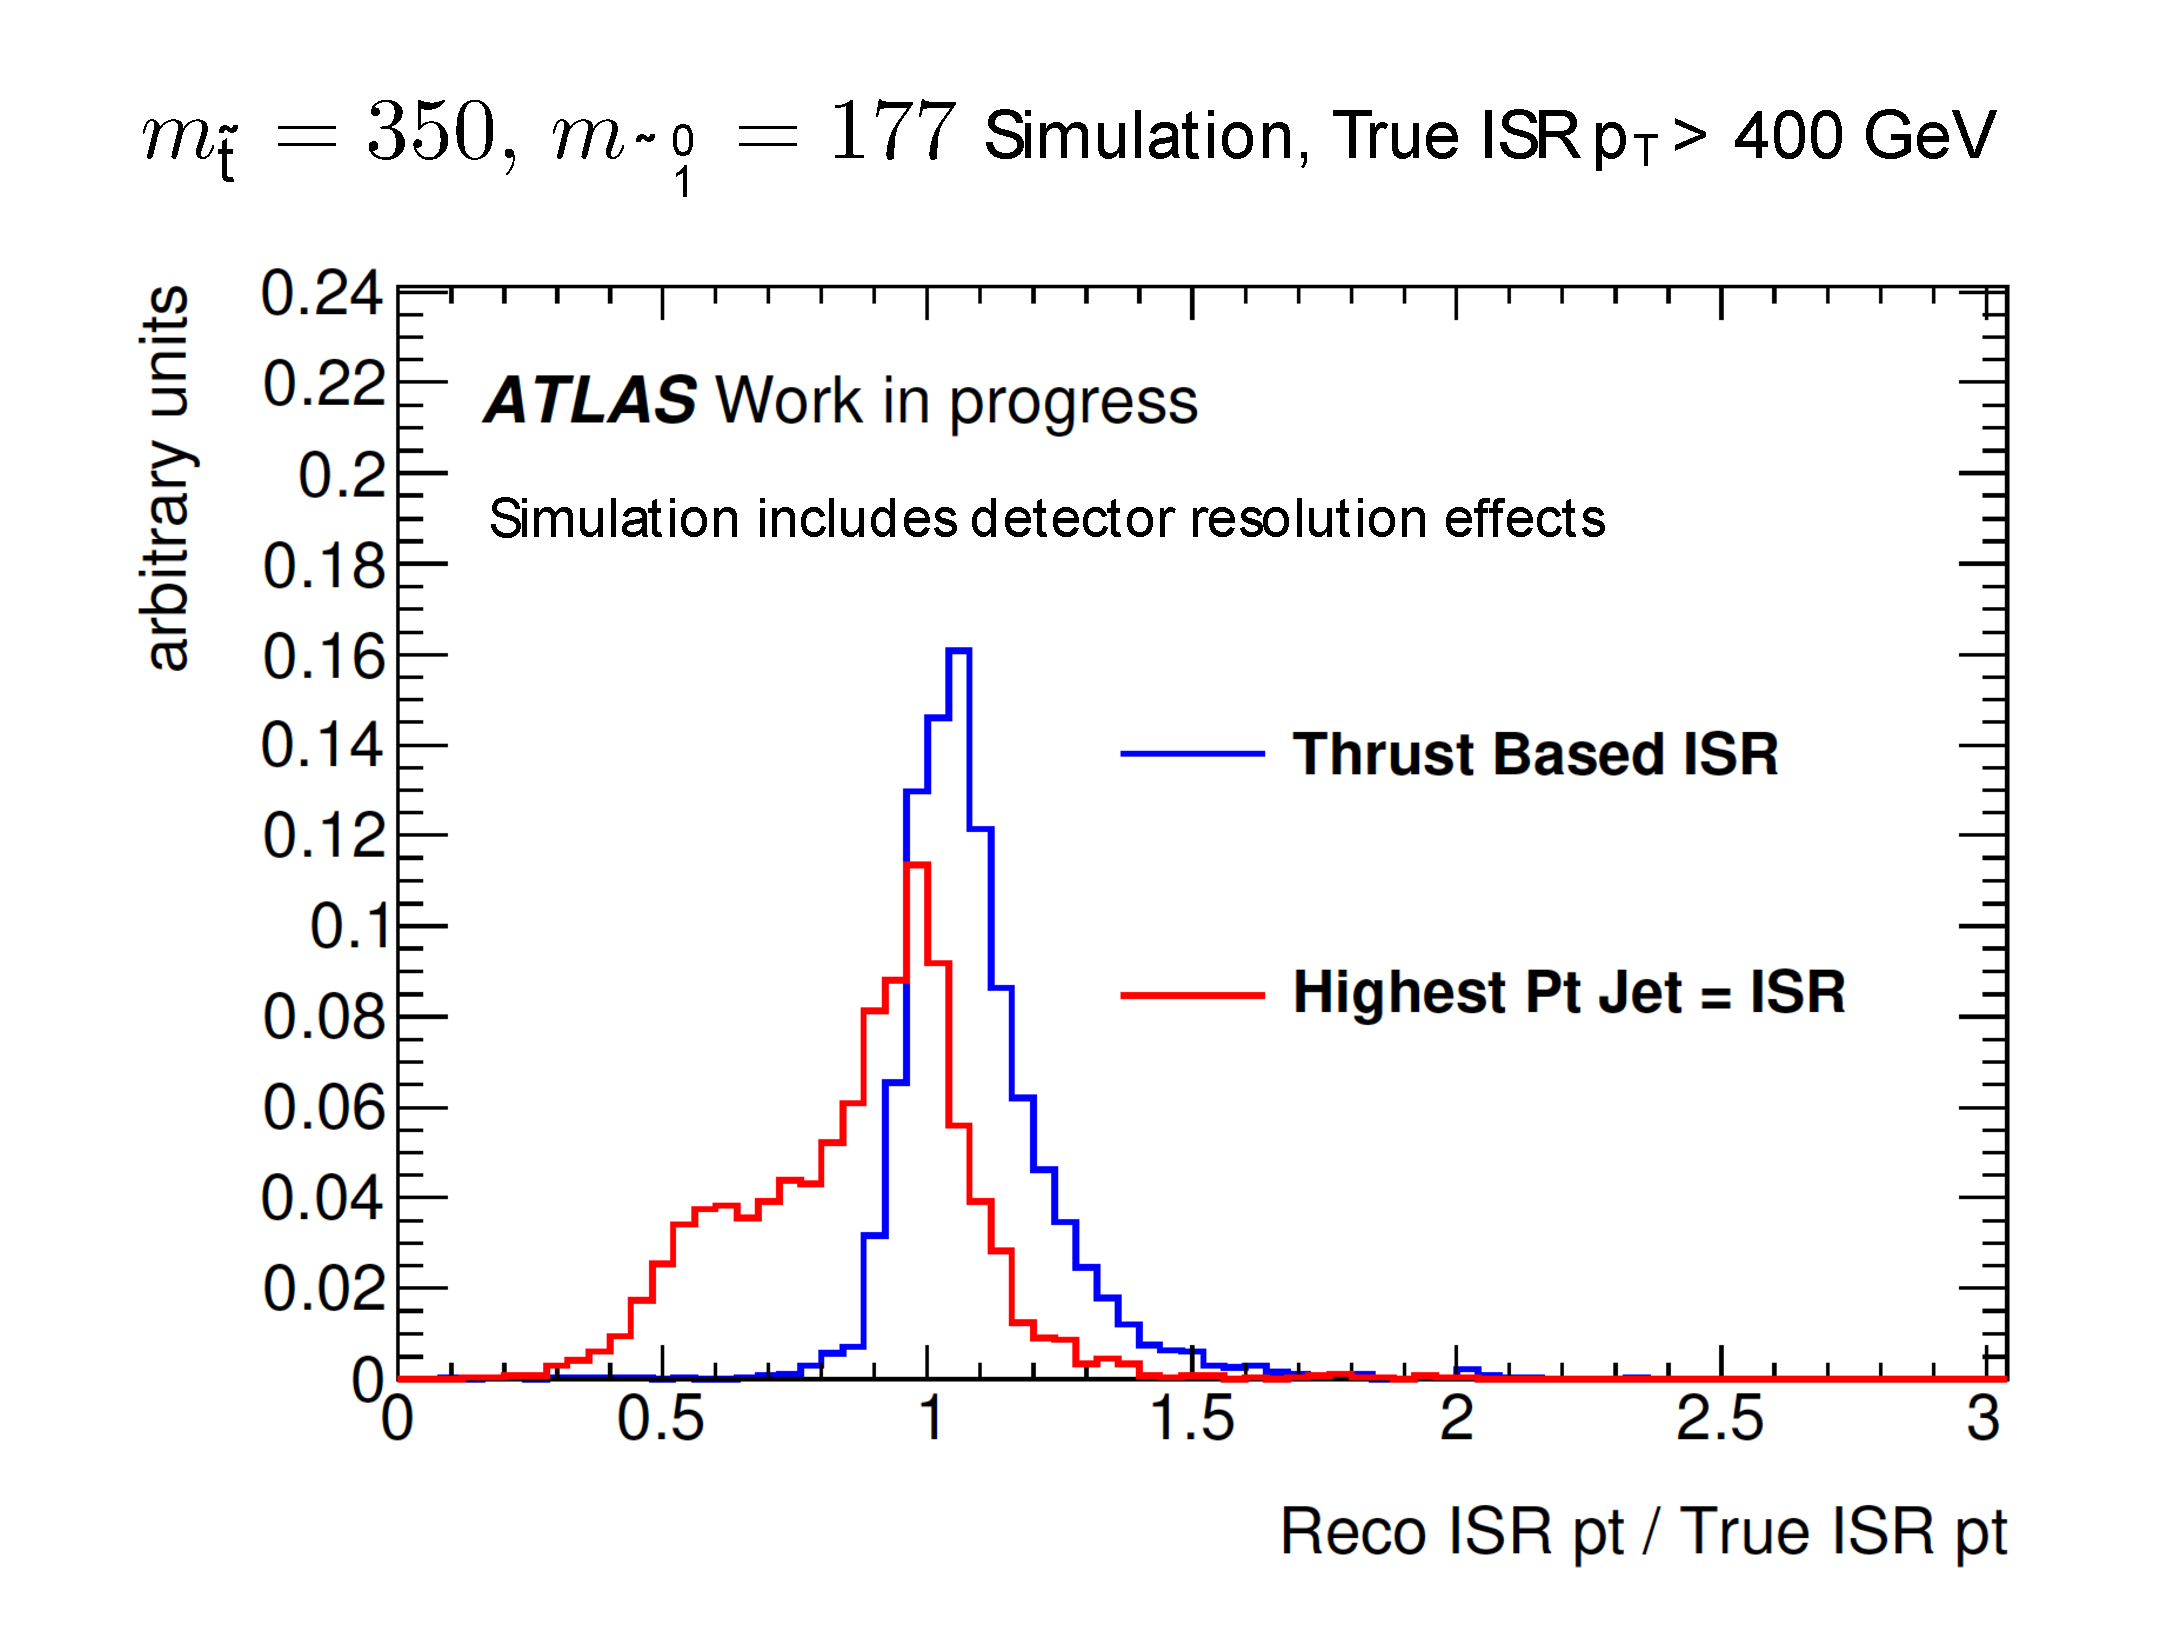
\includegraphics[width=\textwidth]{./figures/strategy/ThrustAlgoEfficiency.eps}
        \caption{ }
    \end{subfigure}
    \begin{subfigure}[b]{0.40\textwidth}
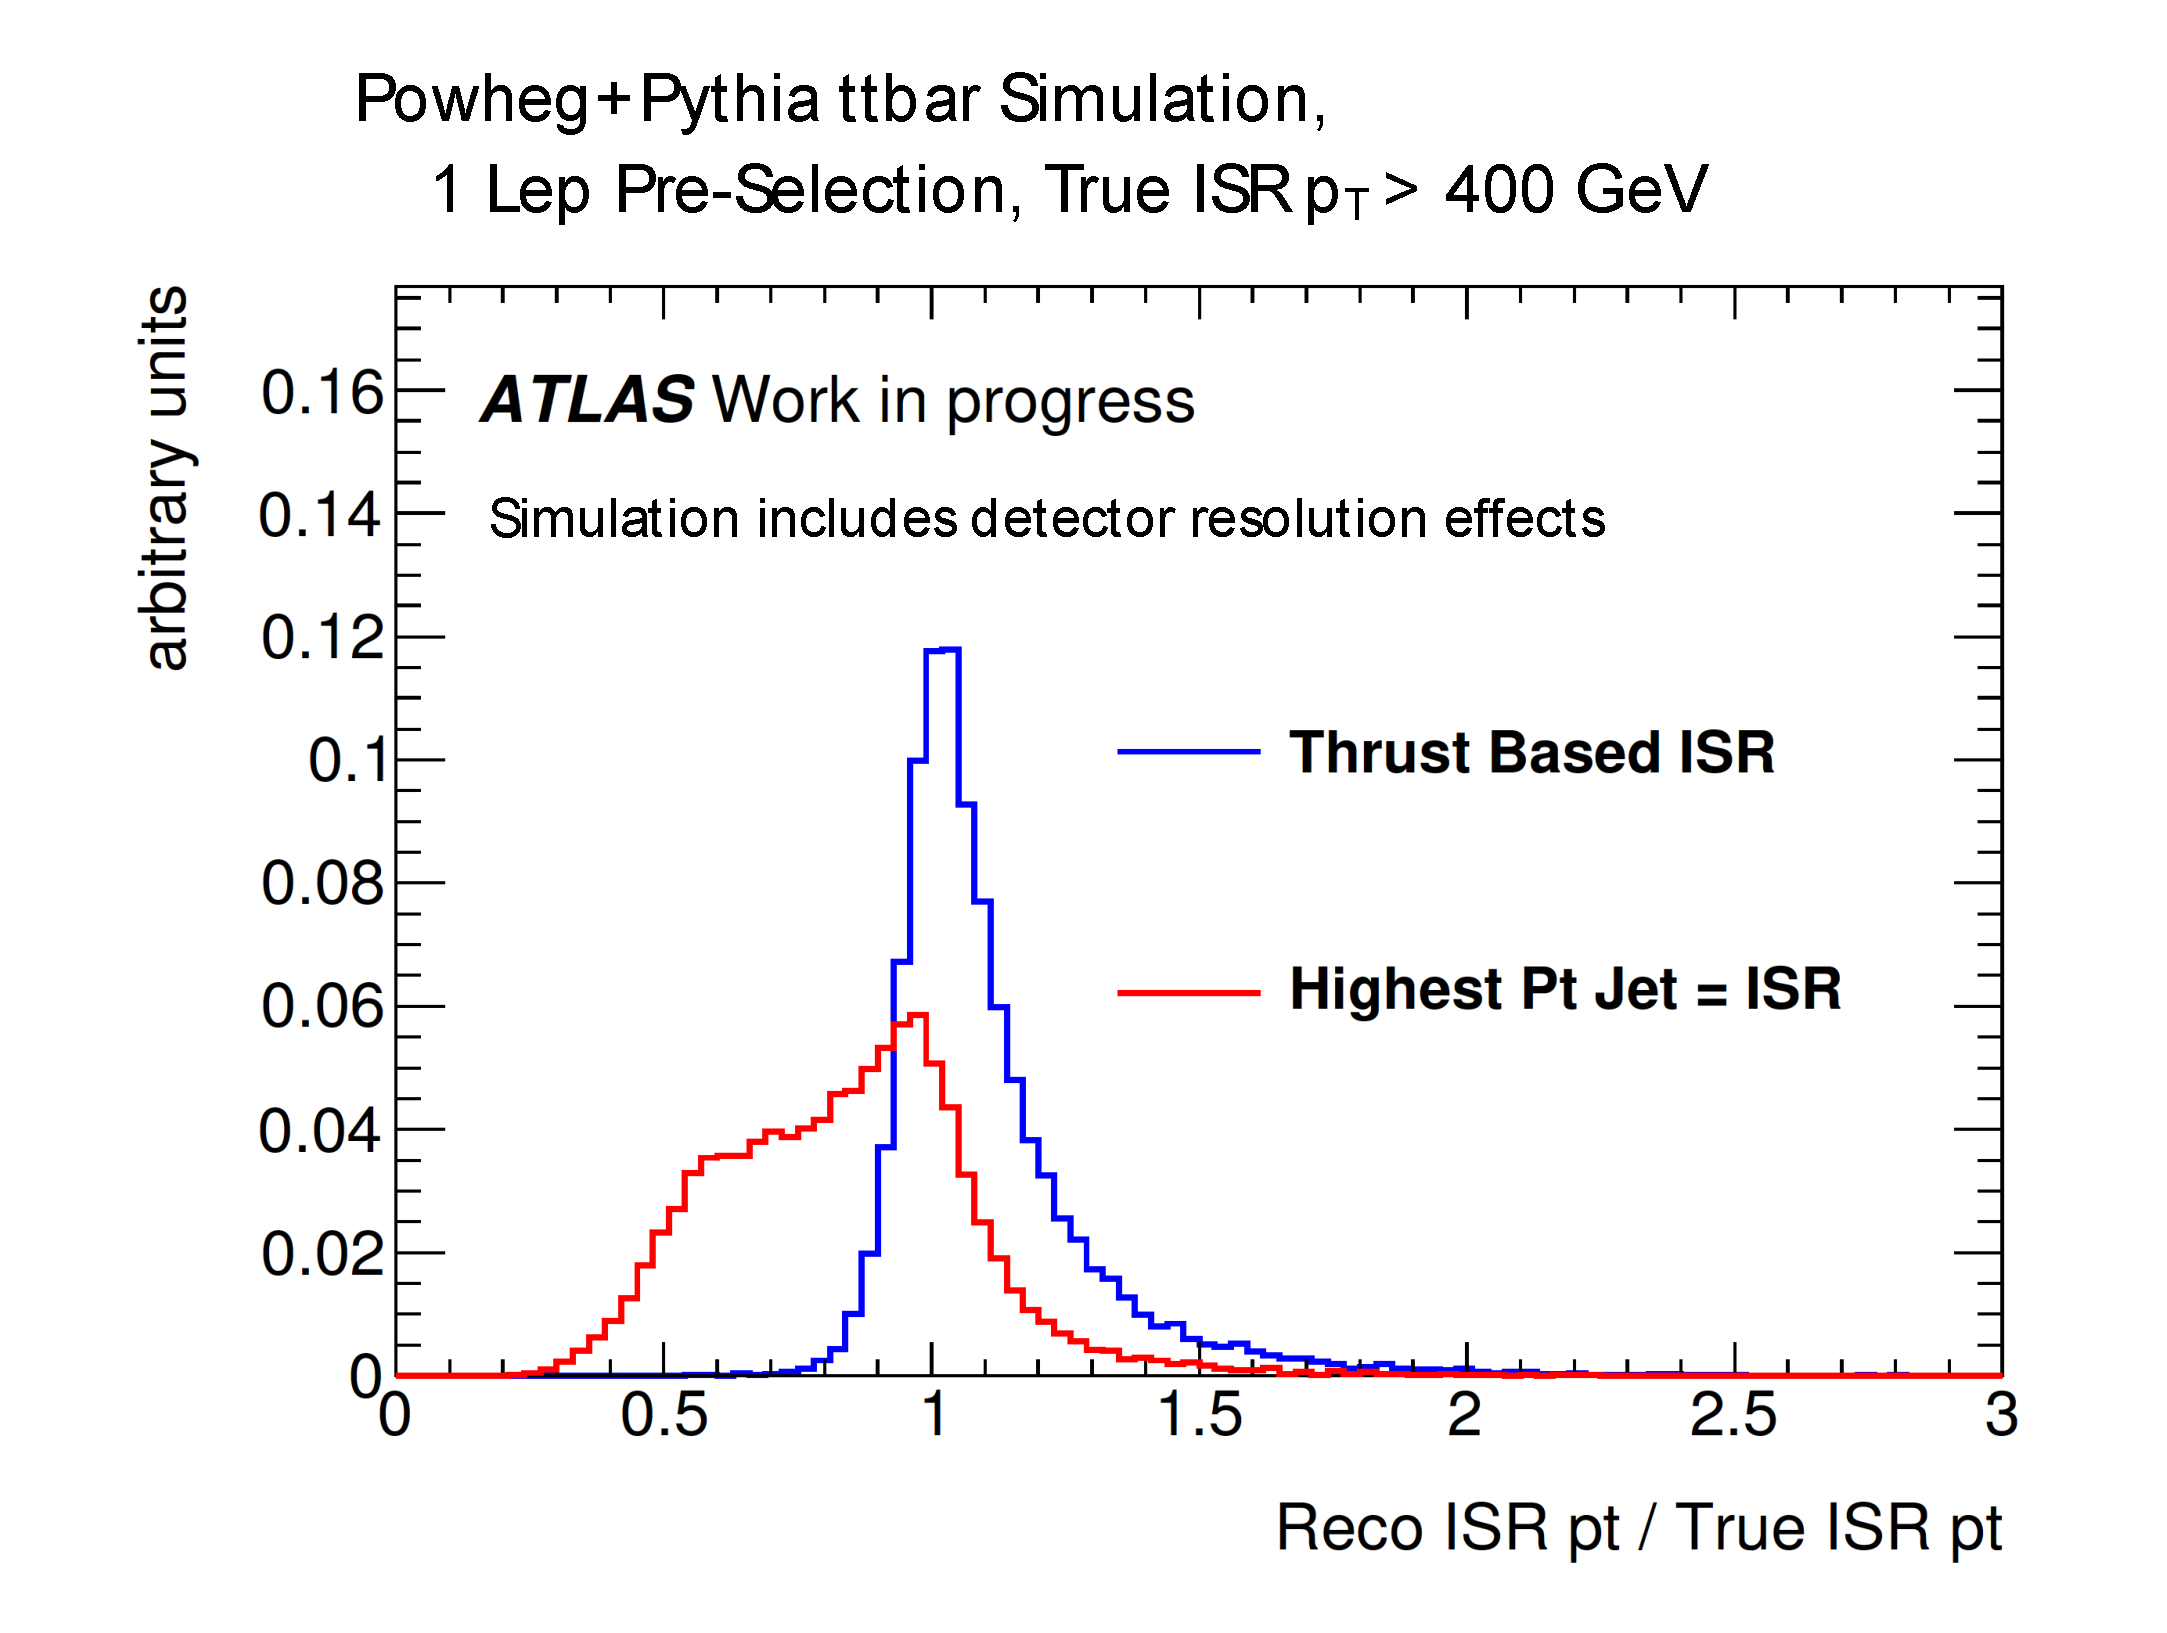
\includegraphics[width=\textwidth]{./figures/strategy/ThrustAlgoEfficiency_ttbar.eps}
        \caption{ }
    \end{subfigure}
\caption[Distributions of the reconstructed ISR $\pt$ over true ISR $\pt$ ratio for stop signal and ttbar background in simulation]{Distributions of the reconstructed ISR $\pt$ over true ISR $\pt$ ratio for stop signal and ttbar background in simulation.  Only events with at least $400$ GeV of true ISR $\pt$ are accepted.  The red distribution is formed when the whole ISR system is equated to just the highest $\pt$ jet.  The blue distribution uses the thrust based ISR identification system. Detector resolution effects are included in the simulation. }
 \label{fig:ISRPerformanceIntro}
\end{figure}

%\indent The ISR based search has allowed us to finally make a definitive statement on the existence of stops in a region with no previous exclusion sensitivity.  Using the $\intlumi$ $\ifb$ 2015 and 2016 $\sqrt{s}=13 \tev$ dataset, we were able to exclude stops in this compressed region with masses between 225 and 600 $\gev$ to 95 percent confidence.  We were able to achieve expected exclusion confidence limits of less then $5 \times 10^{-4}$ for stop masses between 250 and 400 $\gev$.  \\

%\indent The 95\% confidence limit for the analysis is shown in figure \ref{figure.exclusion.All2016}.  The compressed analysis is responsible for the orange region covering the $m_{\stop}-m_{\ninoone} = m_t$ diagonal line.  The compressed analysis also has sensitivity to much of the region between $m_{\stop}-m_{\ninoone} = m_W + m_b$ and $m_{\stop}-m_{\ninoone} = m_t + 30 \gev$.  The sensitivity to this diagonal line complements the two lepton search in purple to the left and the zero lepton high mass splitting search to the right.  \\

%\begin{figure}[h!]
%	\begin{center}
%		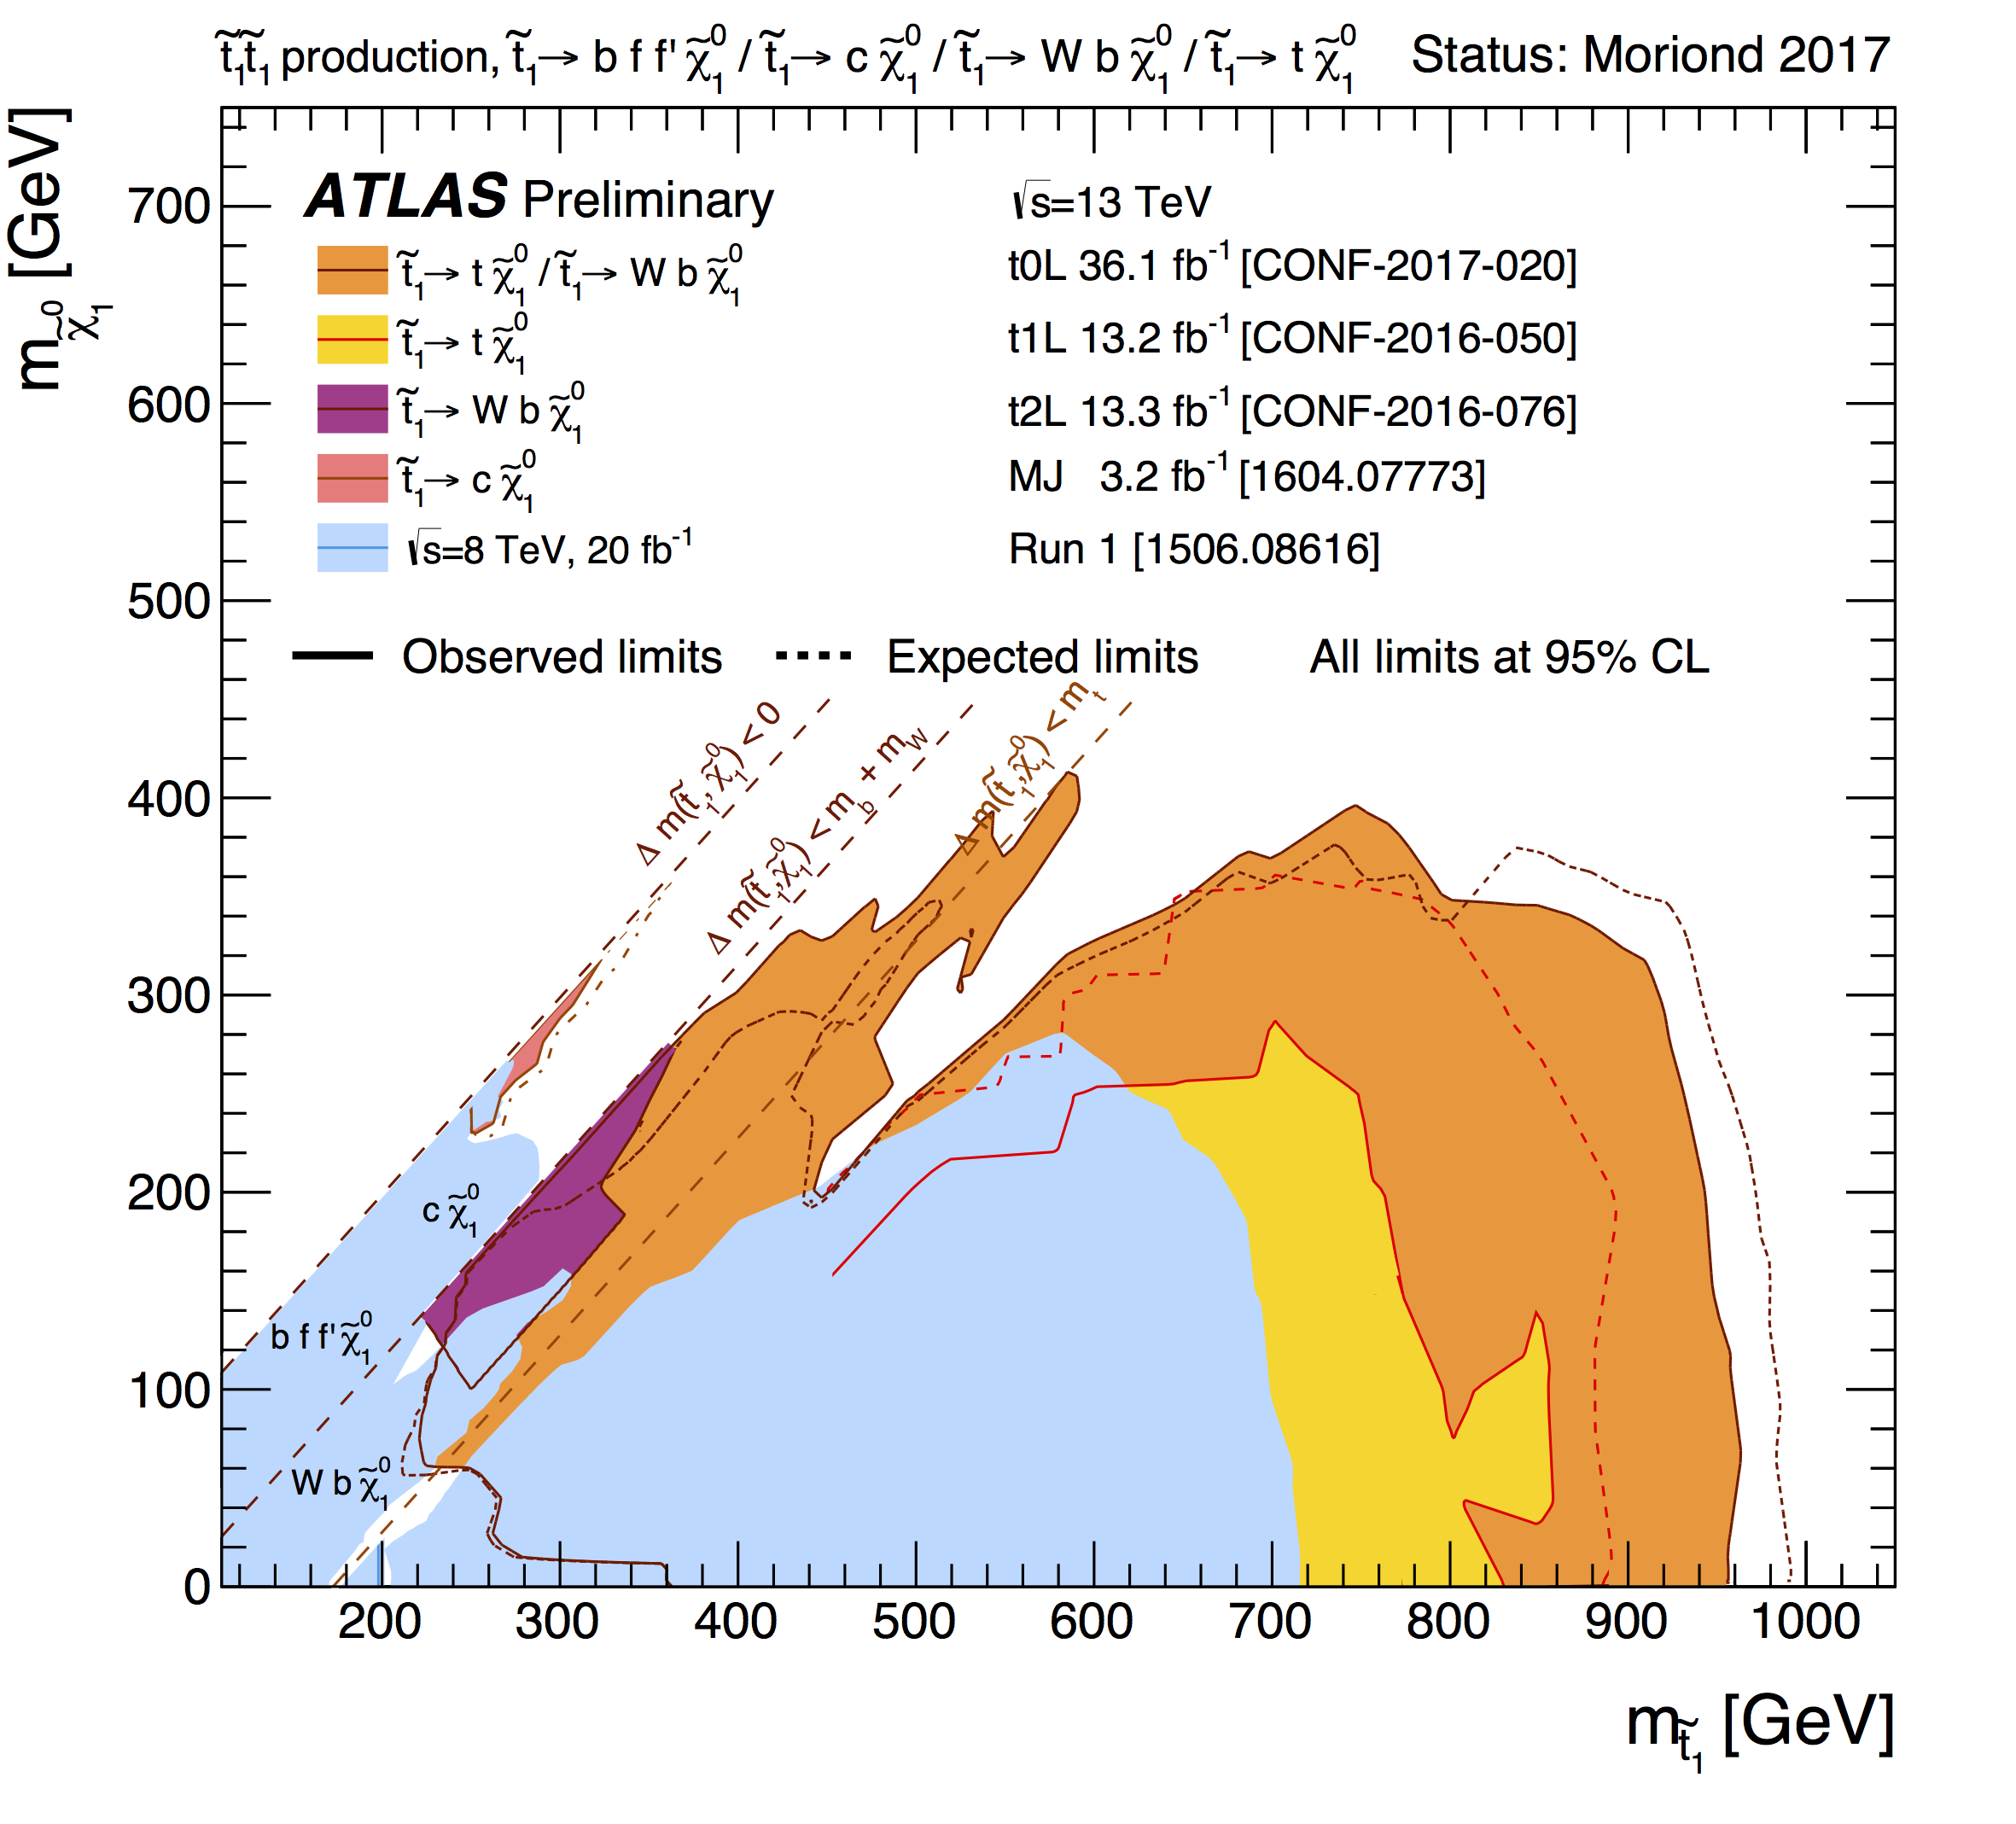
\includegraphics[width=0.85\textwidth]{figures/8TeV/ATLAS_SUSY_Stop_tLSP.png}
%		\caption[95\% confidence limit on stop parameter space resulting from all ATLAS stop searches on the 2015+2016 dataset]{95\% confidence limit on stop parameter space resulting from all ATLAS stop searches on the 2015+2016 dataset.  The compressed analysis is responsible for the orange region covering much of the $m_{\stop}-m_{\ninoone} = m_t$ diagonal line.  The compressed analysis also has sensitivity to much of the region between $m_{\stop}-m_{\ninoone} = m_W + m_b$ and $m_{\stop}-m_{\ninoone} = m_t + 30 \gev$.  The compress analysis covers the region between the 2 lepton analysis in purple and zero lepton high mass splitting search that is also in orange and covers stop mass to 950 $\gev$.  8 $\tev$ ATLAS results are shown in light blue for comparison.  }
%		\label{figure.exclusion.All2016}
%	\end{center}
%\end{figure}

\indent The methods demonstrated in this thesis can be applied to other compressed region searches and searches involving ISR such as dark matter searches.  The accurate ISR identification algorithm can also directly measure the amount of ISR produced in conjunction with SM particles. Potential applications include measuring the SM ttbar ISR $\pt$ spectrum. \\

\indent  The increase in center-of-mass energy from 8 to 13 TeV translates to approximately an order of magnitude increase in the production cross section of heavy sparticles with strong ISR.  The 13 TeV dataset presents a golden opportunity to search for many experimentally difficult physics processes that need a boost from strong ISR in order to be detected.  This ISR based approach allowed us to finally make a definitive statement on the existence of stops in a region with no previous exclusion sensitivity.  \\

\indent The thesis is organized as follows.  Chapter \ref{chap:motivation} presents an overview of the standard model and theoretical motivations for supersymmetry. Chapter \ref{chap:AnaStrategy} concerns the general strategy used in SUSY searches targeting regions with large mass splittings and the general strategy of using ISR to separate signal from background in compressed regions.  \\

\indent Chapter \ref{chap:Exp} describes the experimental setup of the LHC accelerator and ATLAS detector.   Chapter \ref{chap:reconstruction} and chapter \ref{chap:trigger} details the reconstruction and calibration of physics objects at ATLAS the ATLAS trigger system.  \\

\indent The physics objects used in the analysis are defined in chapter \ref{chap:objects}.  The Monte Carlo simulations of stop signal and SM background are described in Chapter \ref{chap:MCSimulation}.  \\ 

\indent We present the new thrust based ISR identification algorithm in chapter \ref{chap:jigsaw}.  The algorithm is explained in context of a more general set of algorithms that uses exterminations to classify objects called Recursive Jigsaw Reconstruction.  The performance of the ISR identification algorithm is also demonstrated on both signal and background. \\

\indent Chapter \ref{chap:data} - \ref{chap:SignalRegion} describes the 2015 and 2016 LHC dataset that is used for this analysis and the kinematic selections used to define the signal region (SR).  The chapters develop physical intuition on each signal region selection and explain how they reject different background.  \\

\indent The SM backgrounds in the SR are described in detail in chapter \ref{chap:backgrounds}.  This chapter explains the using control regions (CRs) to directly estimate the expected background rates in SR.  The CRs are designed to mimic the background kinematics in SR but are orthogonal to SR and are low expected signal rate.  We directly measure the rate of background in the CRs and use simulation to extrapolate background predictions to the SR. \\

\indent  A large portion of chapter \ref{chap:backgrounds} is devoted to building intuition on the unique kinematic properties of each background, especially for the dominant background SM ttbar.  This physical intuition is used to explain the CR design and how the CRs are able to accurately estimate the background rate and minimize systematic uncertainties.  \\

\indent Chapter \ref{chap:Uncertainties} describe each of the experimental and theoretical systematics associated with signal and background.  Systematic uncertainty is divided into two categories; experimental uncertainties due to limitations on detector resolution and theoretical uncertainties on the Monte Carlo simulations. \\

\indent Chapter \ref{chap:statistics} summarizes the statistical methods used to extract the signal strength.  Finally chapter \ref{chap:Results} and \ref{chap:Interpretation} show the results with $\intlumi$ $\ifb$ of $\sqrt{s} = 13 \tev$ data and give an interpretation of the results on select signal models.  \\


%Supersymmetry adds four fermionic coordinates in addition to the usual four bosonic coordinates $(t,x,y,z)$

%Supersymmetry forms an extension to the usual space-time coordinates of $(t,x,y,z)$ and allows for transformations between fermion and bosons.  